\documentclass[11pt,spanish]{article}

% Paquetes
\usepackage{amstext}
\usepackage{amssymb}
\usepackage{amsmath}
\usepackage{babel}
    \addto\shorthandsspanish{\spanishdeactivate{~<>}}
    \decimalpoint
\usepackage[style=iso]{datetime2}
\usepackage{fancyhdr}
\usepackage{float}
\usepackage[T1]{fontenc}
\usepackage[a4paper]{geometry}
    \geometry{verbose,tmargin=3cm,bmargin=2cm,lmargin=2.5cm,rmargin=2.5cm}
\usepackage{graphicx}
\usepackage{hyperref}
\usepackage[utf8]{inputenc}
\usepackage{lastpage}
\usepackage{mathptmx}
\usepackage{tasks}
\usepackage{units}
\usepackage{siunitx}

% dibujos 

\usepackage{tikz}
\usepackage{tikz-dimline}
\usetikzlibrary{calc}
% \usetikzlibrary{math}
\usetikzlibrary{arrows.meta}
\usetikzlibrary{snakes}
\usetikzlibrary{decorations}
\usetikzlibrary{decorations.pathmorphing}
\usetikzlibrary{patterns}

% tipo de fuente 
\usepackage{lmodern}

\pagestyle{fancy}
\lfoot{\small DF, FCEyN, UBA}
\cfoot{\tiny Actualizado el {\today} a las {\DTMcurrenttime}}
\rfoot{\small Pág. {\thepage} de \pageref{LastPage}}

\begin{document}

% Título
    \begin{center}
    \textsc{\large Física 2 (Física) - Cátedra Diana Skigin}
    \par\end{center}{\large \par}
    
    \begin{center}
    \textsc{\large Segundo Cuatrimestre de 2021}
    \par\end{center}{\large \par}
    
    \begin{center}
    \textsc{\large Guía 8: Formación de imágenes}
    \par\end{center}{\large \par}

% Comienzo 
\begin{enumerate}

\section*{Espejos}

% Ejercicio 1

    \item 
    \begin{enumerate}
        \item Demuestre que la imagen dada por un espejo plano de una fuente
        puntual es, sin ninguna aproximación, otra fuente puntual, ubicada
        simétricamente respecto del plano del espejo. Analice los casos que
        corresponden a objetos reales o virtuales.
        
        \item ¿Cuál es la mínima longitud de un espejo plano vertical para que
        un hombre de $1.8$ m de estatura vea su cuerpo entero reflejado? ¿Es
        importante conocer la distancia hombre-espejo? 
    \end{enumerate}

% Ejercicio 2
    
    \item Haga un esquema de un diagrama de rayos localizando las imágenes de
    la flecha que se muestra en la figura. Para un punto de la flecha
    dibuje una porción del frente de ondas emergente y los correspondientes
    frentes reflejados.
    \begin{figure}[H]
        \centering{}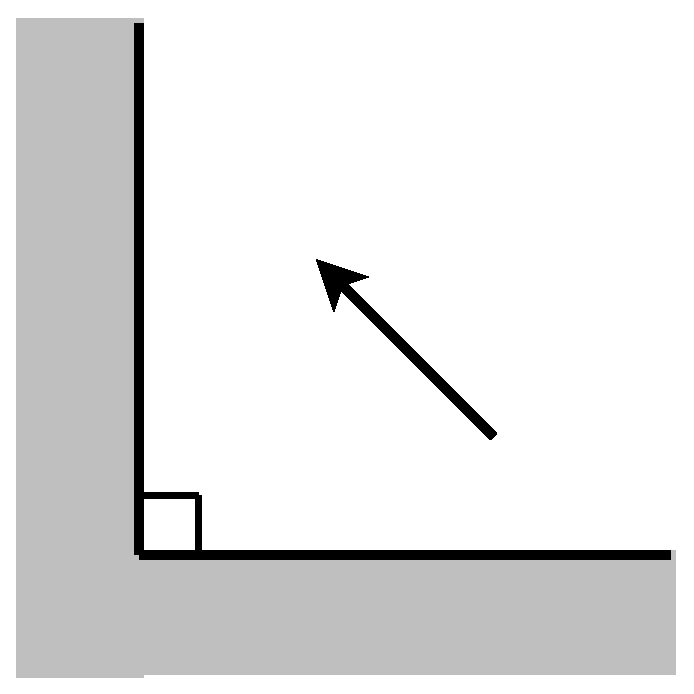
\includegraphics[clip,scale=0.25]{figs/ej3-11}
    \end{figure}

% Ejercicio 3
    
    \item Dos espejos planos forman un ángulo $\alpha$ como lo indica la figura.
    \begin{figure}[H]
        \centering{}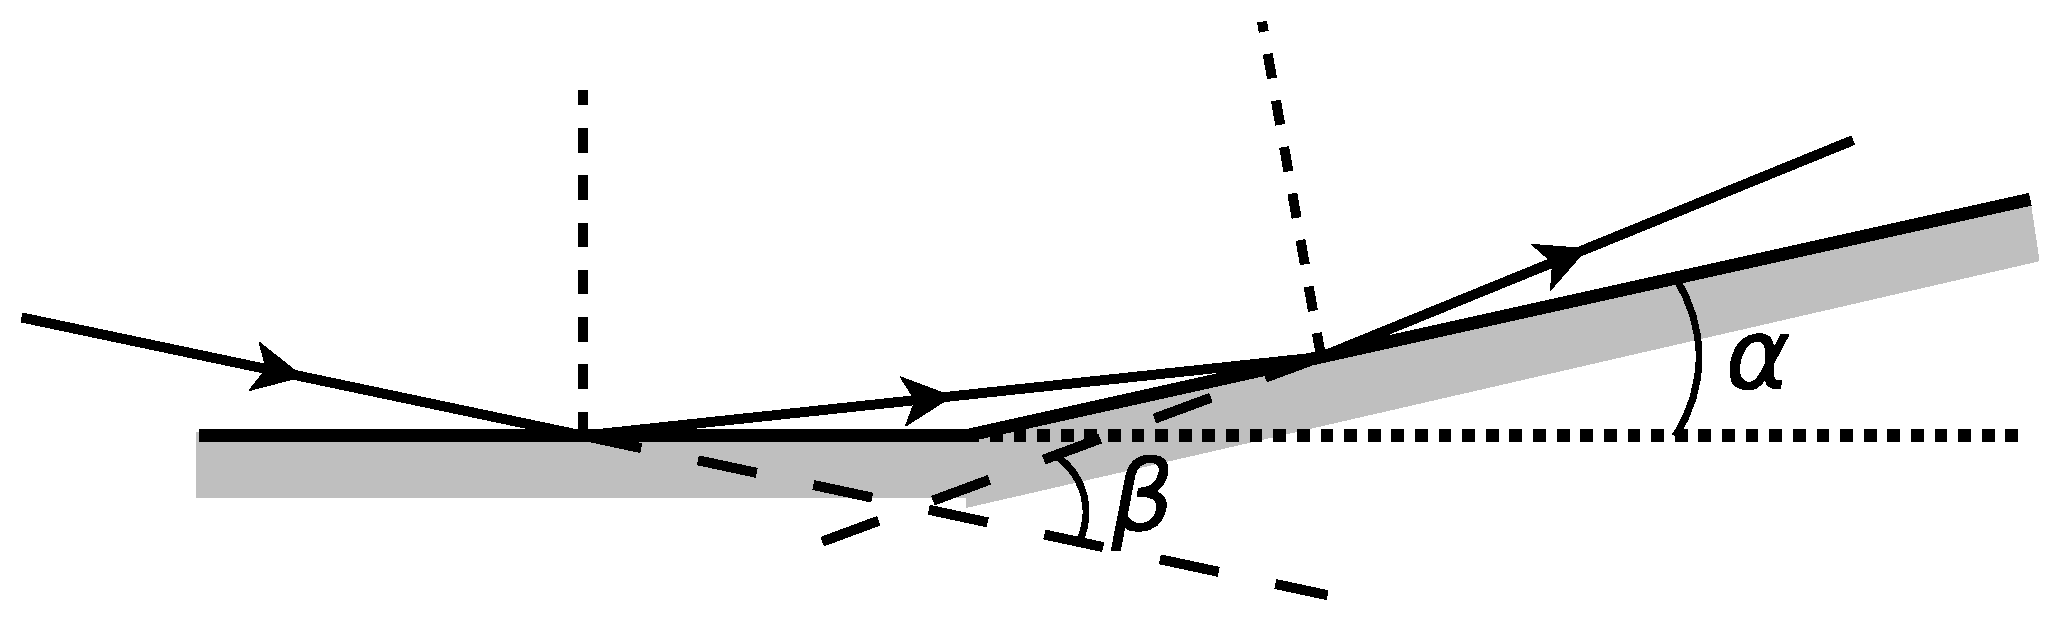
\includegraphics[clip,scale=0.25]{figs/ej3-12}
    \end{figure}
    
    \begin{enumerate}
        \item Un rayo de luz contenido en un plano perpendicular a la
        intersección de los espejos incide sobre uno de ellos, se refleja e
        incide en el otro (ver figura). Calcule el ángulo que forman los rayos
        incidente y emergente.
    
        \item Suponga la misma geometría que en (a) pero ahora iluminada por una
        fuente puntual, demuestre que las imágenes se encuentran sobre una
        circunferencia con centro en el vértice de los espejos. En el caso
        en que la fuente está ubicada de tal modo que sólo se producen dos
        imágenes, y que el ángulo es muy pequeño, calcule la distancia entre
        ellas (espejos de Fresnel).
    \end{enumerate}
    
\section*{Dioptras}

% Ejercicio 4

    \item 
    \begin{enumerate}
        \item Demuestre que un haz homocéntrico (i.e., esférico) de pequeña
        abertura que incide casi normal sobre una dioptra plana, da lugar a otro
        haz homocéntrico. Considere los casos de objetos reales (el haz proviene
        de una fuente puntual) y virtuales (el haz converge hacia un punto).

        \item Una moneda se encuentra en el fondo de un vaso que contiene agua
        hasta una altura de 5 cm ($n_\text{agua}=1.333$). Un observador la mira
        desde arriba, ¿a qué profundidad la ve?

        \item Estimar la máxima abertura de un haz homocéntrico, para que la
        posición de la imagen, formada por una única superficie plana, quede
        determinada con un error del 2\%. 
        
        \item Usando los resultados anteriores, demuestre que un haz
        homocéntrico de pequeña abertura, al atravesar una lámina de caras
        paralelas, da lugar, en primera aproximación, a otro haz homocéntrico.
        Halle la posición de las sucesivas imágenes. 
        
    \end{enumerate}

% Ejercicio 5
    
    \item Haciendo uso de la figura, de la ley de Ibn Sahl-Snell y del hecho de
    que en la aproximación paraxial $\alpha\approx\sin\alpha\approx\tan\alpha$
    (lo mismo pasa con $\beta$ y $\varphi$):

    \begin{figure}[H]
        %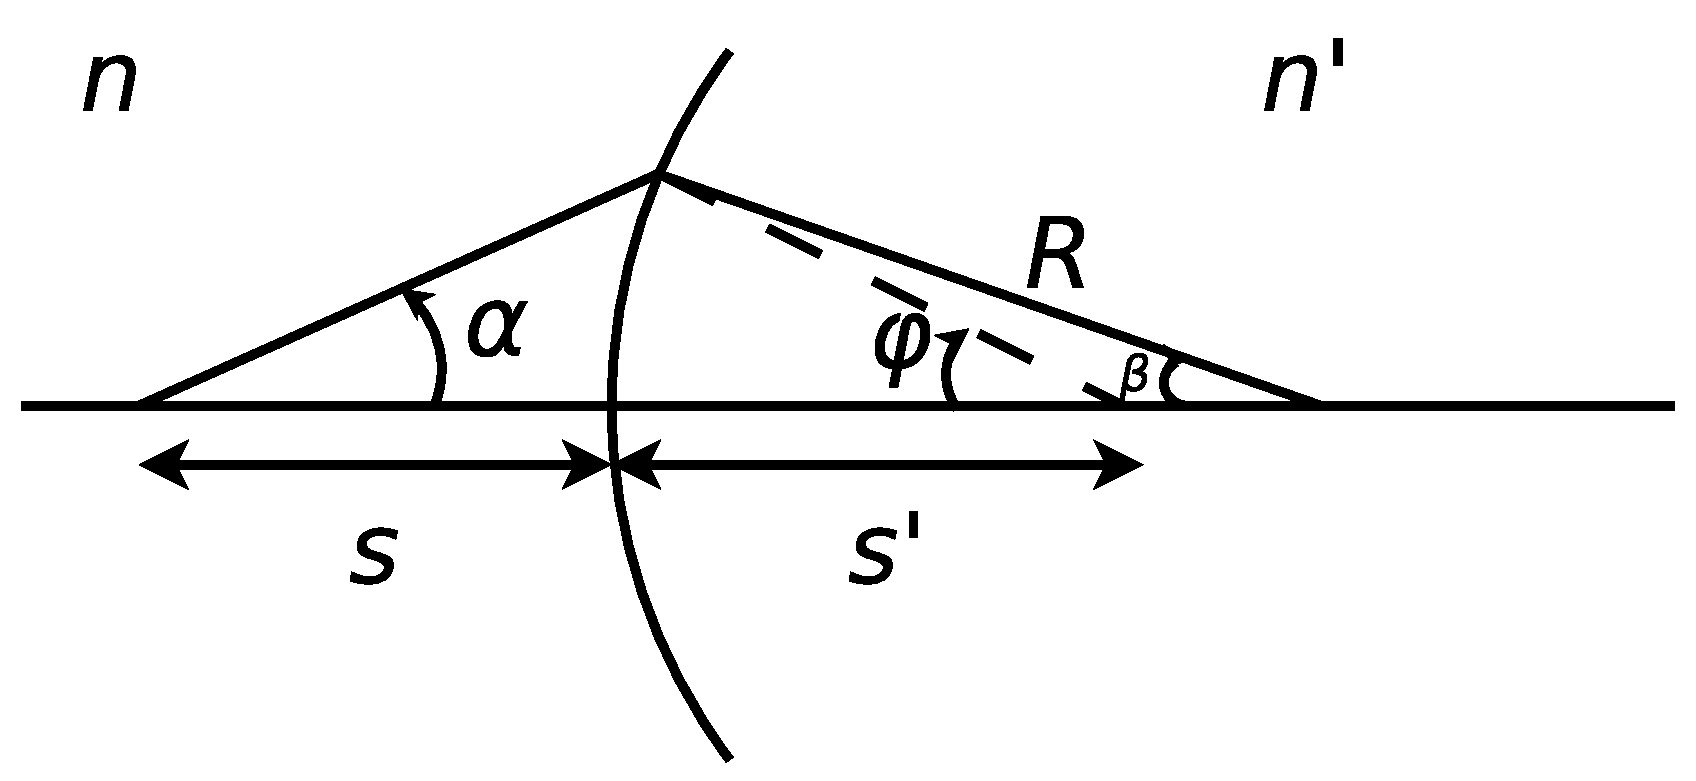
\includegraphics[clip,scale=0.25]{figs/ej3-15}
        \centering{}
        \begin{tikzpicture}
        	\def \arcoDioptra{30};
        	\def \radioDioptra{3};
        	\coordinate (origenDioptra) at (-1,0);
        	\coordinate (so) at (-2,0);
        	\coordinate (centroDioptra) at (\radioDioptra,0);
        	\coordinate (si) at (5,0);
        	\coordinate (interseccionDioptra) at ({2 - \radioDioptra*cos(25)},{\radioDioptra*sin(25)});
        	\draw [thin, dashed] (-2.5,0) -- (5.5,0);% node [midway, anchor=north] {eje óptico} ;
        	\draw [ultra thick] (origenDioptra) arc(180 : 180 - \arcoDioptra : \radioDioptra);
        	\draw [ultra thick] (origenDioptra) arc(180 : 180 + \arcoDioptra : \radioDioptra);
        	\draw [thin, -LaTeX] (centroDioptra) -- (interseccionDioptra) node [midway, below, rotate = -18] {\(R\)};
        	\draw [-latex] ($(centroDioptra) - (1,0)$) arc(180 : {180-atan{0.34}} : 1) node [midway, left] {$\varphi$};
        	\draw [thick, blue, -LaTeX] (so) -- (interseccionDioptra);
        	\draw [-latex] ($(so) + (0.6,0)$) arc(0 : {atan{0.57}} : 1) node [midway, right] {$\alpha$};
        	% \dimline[line style ={line width=0.7}]{($(so) - (0,0.5)$)}{($(origenDioptra) - (0,0.5)$)}{$s$};
        	\dimline[line style ={line width=0.7},extension start length=-0.5,extension end length=-0.1]{($(so) - (0,0.5)$)}{($(origenDioptra) - (0,0.5)$)}{$s$};
        	\draw [thick, blue, LaTeX- ] (si) -- (interseccionDioptra);
        	\draw [-latex] ($(si) - (1.7,0)$) arc(180 : {180-atan{0.4}} : 1) node [midway, left] {$\beta$};
        	% \dimline[line style ={line width=0.7}]{($(origenDioptra) - (0,0.5)$)}{($(si) - (0,0.5)$)}{$s'$};
        	\dimline[line style ={line width=0.7},extension start length=-0.1,extension end length=-0.09]{($(origenDioptra) - (0,0.5)$)}{($(si) - (0,0.5)$)}{$s'$};
        \end{tikzpicture}
        
    \end{figure}
    
    \begin{enumerate}
    
        \item Obtenga la ecuación de las dioptras esféricas, que establece lo
        siguiente:
        \[
        \frac{n'}{s'}\mp\frac{n}{s}=\frac{(n'-n)}{R}
        \]
        
        Discuta el doble signo, asociándolo con la convención de signos que se
        utilice (Newton o Descartes).
    
        \item A partir de un gráfico de $s'$ vs $s$, analice para qué posiciones
        de los objetos reales las imágenes son reales o virtuales, directas o
        invertidas y lo mismo para objetos virtuales. Analice todos los casos
        posibles para dioptras convergentes y divergentes. ¿Cómo determinaría
        los focos a partir del gráfico?
    
        \item ¿Pueden ser iguales las dos distancias focales de una dioptra?
        ¿Depende su respuesta de la convención de signos empleada?

    \end{enumerate}

% Ejercicio  6

    \item La esfera de vidrio de la figura, de 1 cm de diámetro, contiene una
    pequeña burbuja de aire desplazada $0.5$ cm de su centro. Hallar
    la posición y el aumento de la burbuja cuando se la observa desde
    \emph{A} y cuando se la observa desde \emph{B}.

    \begin{figure}[H]
        \centering{}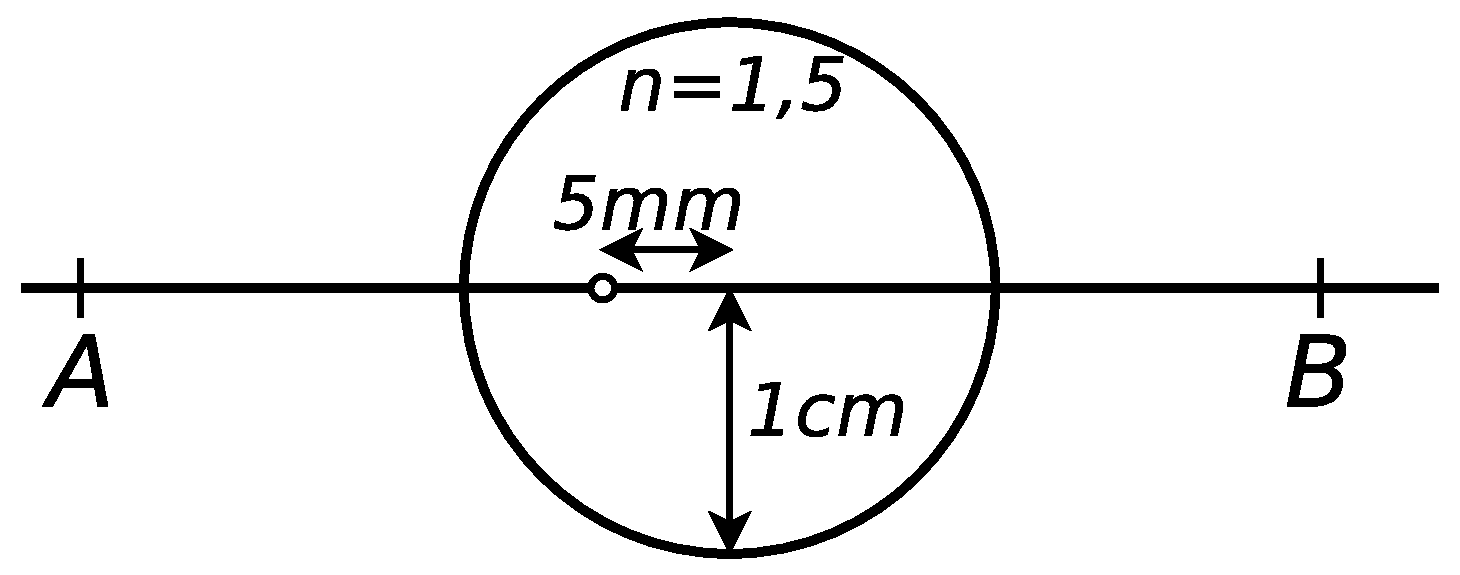
\includegraphics[clip,scale=0.25]{figs/ej3-17}
    \end{figure}

% Ejercicio 7

    \item Calcular la posición y tamaño de la imagen formada por cada una de las
    dioptras, y especificar si son reales o virtuales para el caso de la figura.
    Hacer un trazado de rayos a escala.

    \begin{figure}[H]
        \centering{}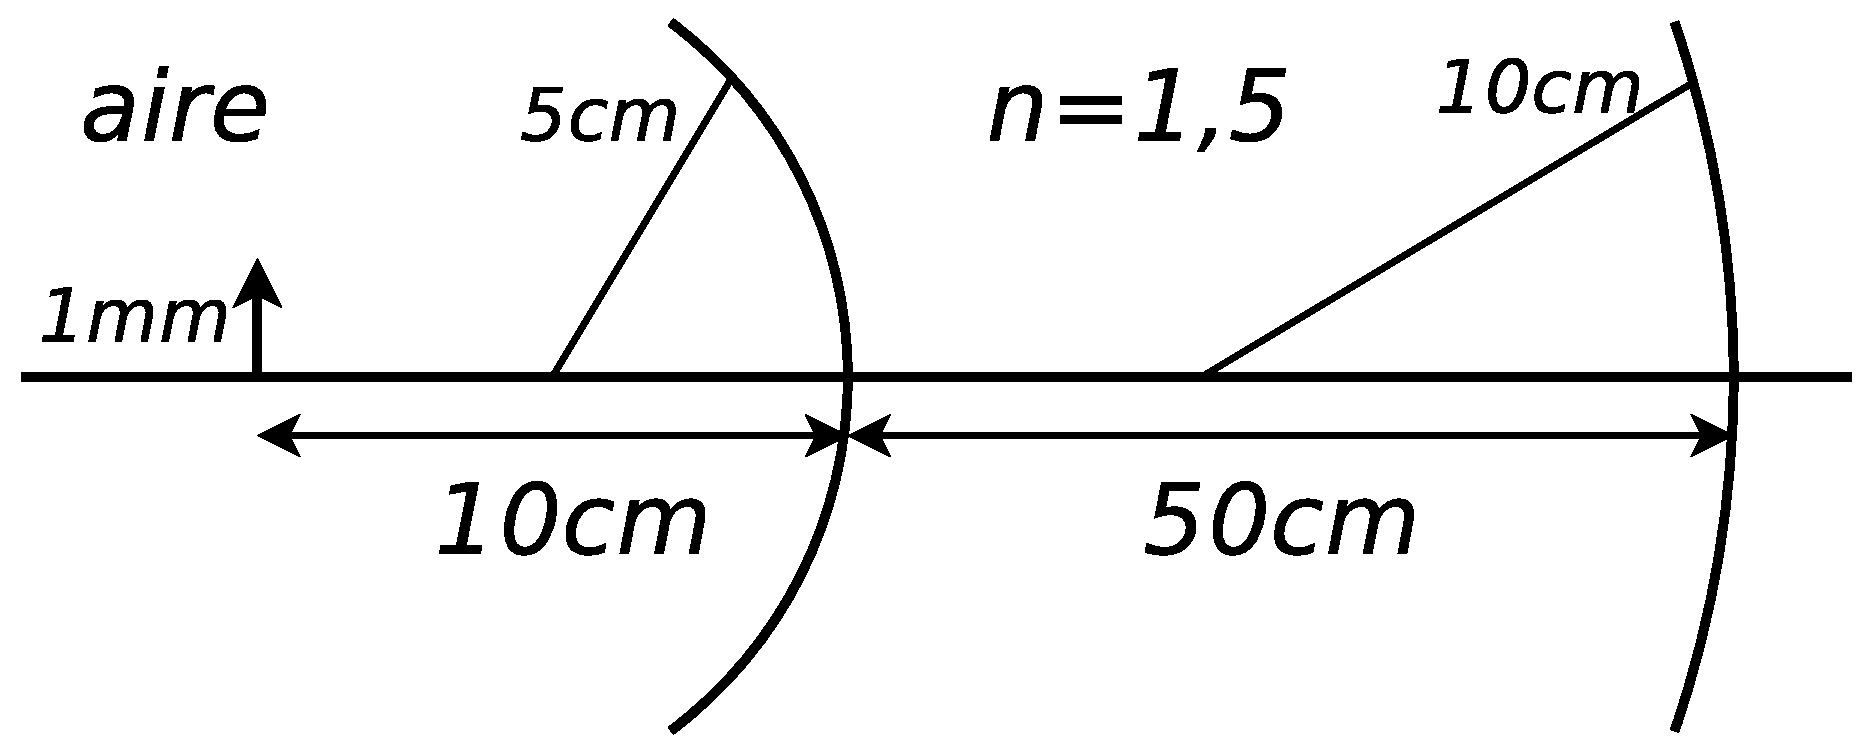
\includegraphics[clip,scale=0.25]{figs/ej3-16}
    \end{figure}


% Ejercicio 8

    \item 
    \begin{enumerate}
        \item Partiendo de la ecuación de las dioptras, obtenga la ecuación de
        los espejos esféricos. 
        
        \item ¿Cómo se modifica la distancia focal de un espejo esférico si se
        lo sumerge en agua? ¿Y en otro medio diferente?
        
        \item Calcule la distancia focal de un espejo esférico cóncavo, sabiendo
        que produce una imagen cuyo tamaño es el doble del tamaño del objeto,
        siendo la distancia objeto--imagen de 15 cm.
    \end{enumerate}

\section*{Lentes delgadas}

% Ejercicio 9

    \item 
    \begin{enumerate}
        \item A partir de la ecuación de la dioptra, considerando dos dioptras
        esféricas tal que la separación entre ellas sea mucho menor que las
        restantes longitudes involucradas, deduzca la ecuación para las lentes
        delgadas.
        
        \item Analice de qué depende la convergencia o divergencia de una lente.
        
        \item Grafique $s'$ vs $s$ para lentes convergentes y divergentes,
        analice el aumento y la posición de los objetos (en particular objeto en
        el foco y objeto en infinito) y de las imágenes.
        
        \item ¿Pueden ser iguales (en módulo) los focos de una lente? En ese
        caso, ¿representan el mismo punto en el espacio? ¿Qué interpretación
        tiene una distancia focal negativa en cada convención de signos?
        
        \item Demuestre que la menor distancia objeto--imagen es $4f$, si la
        lente está inmersa en un único medio.
        
        \item Dibuje los frentes de onda incidente, refractado por la primera
        dioptra y refractado por la segunda.
        
    \end{enumerate}

% Ejercicio 10    
    
    \item Determine:
    \begin{itemize}
        \item la posición de los focos objeto e imagen.
        \item la potencia óptica en dioptrías $\mathcal{D} = \frac{1}{f}$,
        con \(f\) expresada en \si{\metre}.
        \item El aumento \(M\) expresado popularmente en unidades de $\times$
        (e.g. $4\times$), como \(M = \SI{0.25}{\metre} \mathcal{D} + 1\).
    \end{itemize}
    para los siguientes casos:
    \begin{enumerate}
        \item Lente plano--cóncava ($n=1.5$)
        cuyo radio de curvatura es $10$ cm. Determine su potencia en dioptrías.
        
        \item Lente de vidrio ($n=1.6$) sumergida en agua, sabiendo que su
        distancia focal en el aire es de 20 cm.
        
        \item Lente biconvexa con $R_{1}=R_{2}=10$ cm, construida con un vidrio
        de índice $1.5$, inmersa entre aire de un lado y un líquido de índice
        $1.7$ del otro. 
        
        \item Misma lente que en el caso anterior si i) está inmersa sólo en
        aire, ii) está inmersa en el medio de índice $1.7$. Discuta cómo se
        modifica la convergencia en cada caso.
    \end{enumerate}

% Ejercicio 11

    \item
    \begin{enumerate}

        \item Se coloca un objeto a $18$ cm de una pantalla, ¿en qué puntos
        entre la pantalla y el objeto se puede colocar una lente delgada
        convergente de distancia focal $4$ cm, para que la imagen del objeto
        esté sobre la pantalla? ¿Qué diferencia hay entre ubicarla en una u otra
        posición?
        
        \item Un objeto se halla a distancia fija de la pantalla. Una lente
        delgada convergente, de distancia focal $16$ cm, produce imagen nítida
        sobre la pantalla cuando se encuentra en dos posiciones que distan entre
        sí $60$ cm. ¿Cuál es la distancia objeto--pantalla?
    \end{enumerate}

% Ejercicio 12

    \item Considere una lente inmersa en dos medios diferentes como se indica en
    la figura
    
    \begin{figure}[H]
        \centering{}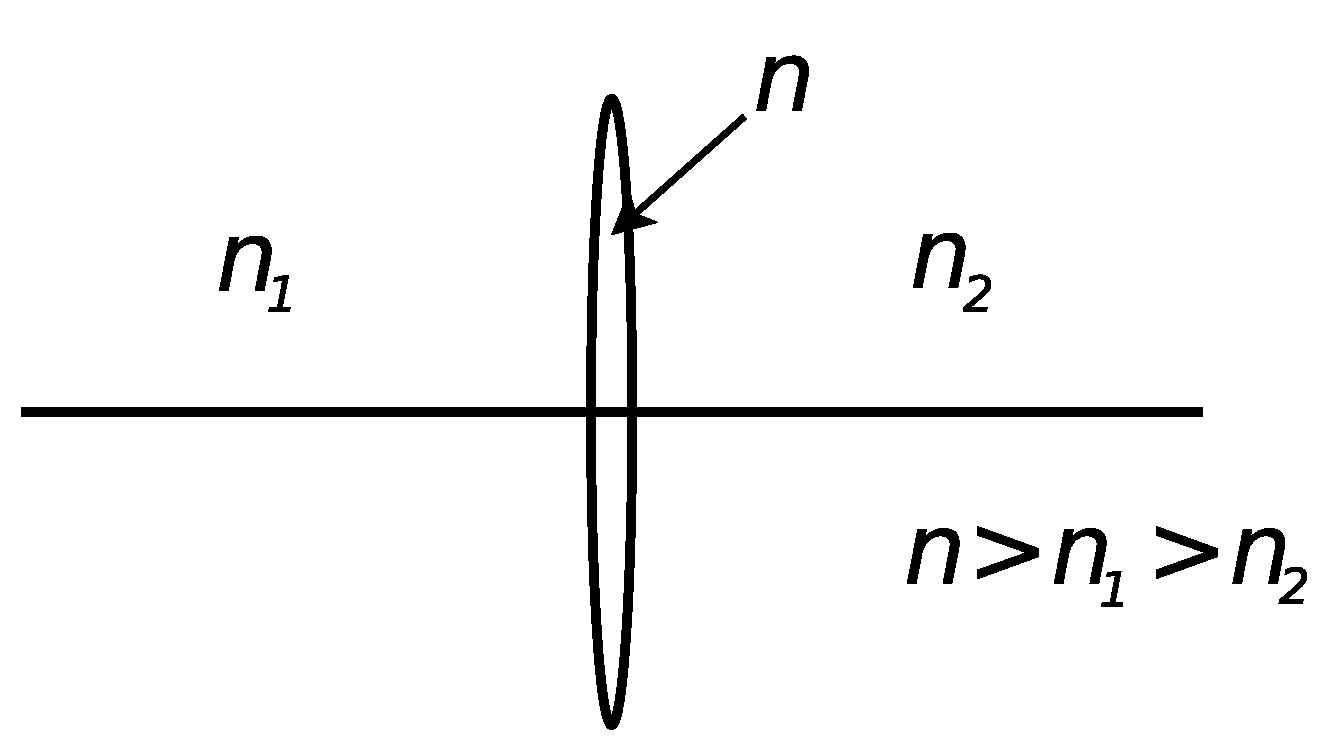
\includegraphics[clip,scale=0.25]{figs/ej3-25}
    \end{figure}
    
    \begin{enumerate}
    
        \item Determine la posición del foco objeto y del foco imagen.
    
        \item Verifique las reglas de trazado de rayos para rayos que atraviesan
        alguno de los focos.
    
        \item Indique en qué punto del eje óptico debe incidir un rayo para que
        atraviese la lente sin desviarse. Exprese el resultado en función de la
        distancia focal objeto y de los índices de refracción.
    \end{enumerate}

% Ejercicio 13

    \item Una lente delgada convergente, de distancia focal 30 cm, se coloca
    $20$ cm a la izquierda de otra lente delgada divergente de distancia focal
    $50$ cm. Para un objeto colocado a $40$ cm a la izquierda de la
    primera lente determine la imagen final. ¿Cuál es el aumento? La imagen,
    ¿es real o virtual?, ¿es directa o invertida?

\section*{Instrumentos ópticos}

% Ejercicio 14
    
    \item 
    \begin{enumerate}
        \item Determine el radio de curvatura de una lupa equiconvexa ($n=1.5$)
        para que su aumento sea $10 \times$. ¿Dónde se encuentra la imagen, y
        el objeto?
        
        \item Calcule el aumento de la lupa descripta en (a) cuando la imagen se
        encuentra a la distancia de visión clara. Discuta las ventajas y
        desventajas de esta opción.
    \end{enumerate}

% Ejercicio 15
    
    \item Un microscopio consta de un objetivo de 4 mm de distancia focal y
    de un ocular de $30$ mm de distancia focal. La distancia entre el foco
    imagen del objetivo y el foco objeto del ocular es $g=18$ cm. Calcule:

    \begin{enumerate}
        \item El aumento normal del microscopio.
        
        \item La distancia objeto--objetivo.
        
        \item Sabiendo que el microscopio no cuenta con diafragmas adicionales,
        y que la pupila de salida debe ser real, y del mismo diámetro aproximado
        que la pupila del ojo ($\approx$12 mm), discuta cuál de las dos lentes
        debe ser el diafragma de apertura, cuál debe ser su diámetro y en
        qué posición se halla la pupila de salida.
        
        \item Discuta en qué posiciones colocaría un diafragma de campo, y si esta
        introducción modifica o no la determinación del diafragma de apertura.
    \end{enumerate}

% Ejercicio 16

    \item Un anteojo astronómico utiliza como objetivo una lente convergente
    de $2$ m de distancia focal y $10$ cm de diámetro, y como ocular una lente
    convergente de $4$ cm de distancia focal. Determine:
    \begin{enumerate}
        \item El aumento eficaz.
        \item Las características de la primer imagen de la luna y de la imagen
        final a través del telescopio. La luna subtiende, a ojo desnudo, un
        ángulo de 31'.
        
        \item El largo total del tubo.
        
        \item El mínimo diámetro del ocular para que el objetivo sea diafragma de
        apertura. (Recordar que la luna no es puntual, y por ende hay puntos
        objeto extra-axiales).
        
        \item Suponiendo que el diámetro del ocular sea de 4 cm, la posición y el
        tamaño de la pupila de salida.
        
        \item La posición en que debe colocarse el ojo.
        
        \item La posición en que debe colocarse, de ser posible, un diafragma de
        campo.
        
        \item El mínimo diámetro del posible diafragma de campo para que la imagen
        de la luna se vea completa 
    \end{enumerate}
    
\end{enumerate}

\end{document}

